\clearpage 
\section{Summary}
\label{sec:summary}
Using data samples collected at thirteen center-of-mass energies ranging from 4.600 to 4.951 GeV with the BESSIII detector at BEPCII, we present a measurement of $\Lambda_c^+$ transverse polarization in $e^+e^- \to \Lambda_c^+ \Lambda_c^-$ through a partial wave analysis of $\Lambda_c^+ \to p K^- \pi^+$ decay. The angular distribution parameter $\alpha_0$ and the phase angle difference $\Delta_0$ in the two helicity amplitudes for $e^+e^- \to \Lambda_c^+ \Lambda_c^-$ are obtained at each energy point, as shown in Table~\ref{tab:final-results}. A significance test of $\Lambda_c^+$ transverse polarization is performed, with $\Delta_0$ fixed at 0 for each energy point to calculate the significance value. The most significant $\Lambda_c^+$ transverse polarization is observed at a center-of-mass energy of $\sqrt{s} = 4.68192\ \text{GeV}$, with a statistical significance of 6.7$\sigma$. The maximal values of transverse polarization for each energy points are calculated using Equation~\ref{eq:eq_polar} and shown in Figure~\ref{fig:max_py}. The fit fractions of the intermediate resonances in $\lcp \to p K^-\pi+$ are shown in Table~\ref{tab:final-ff}. Using the branching fraction of $\BR(\lcp \to p K^-\pi+) = (6.26\pm0.29)\%$ in PDG~\cite{Workman:2022ynf}, the branching fractions of $\lcp \to p\bar{K}^*(892)$, $\lcp \to \Delta(1232)^{++}K^-$ and $\lcp \to \Lambda(1520)\pi^+$ are calculated and shown in Table~\ref{tab:final-bf}.

When compared to the other studies conducted at BESIII~\cite{BESIII:2017kqg,BESIII:2023rwv}, our measurements of $\alpha_0$ remain consistent in terms of precision, as outlined in Table~\ref{tab:alpha0-comparison}.
The ratio of electromagnetic form factors $|G_E/G_M|$ are derived and are found to agree well with the previous measurements and theoretical predictions~\cite{Chen:2023oqs}, as shown in the left of Figure~\ref{fig:comp_theory}.
To facilitate the comparison of $\Delta_0$ results with another measurement~\cite{ESIIImemo:LcDecayAsy}, the $\sin\Delta_0$ values listed in Table~\ref{tab:final-results} have been converted into $\Delta_0$ values within the range of [$-\frac{\pi}{2}$, $\frac{\pi}{2}$]. The comparison outcomes, presented in Table~\ref{tab:delta0-compare}, show agreement within 2$\sigma$ of errors. The comparison of $\sin\Delta_0$ between theoretical predictions~\cite{Chen:2023oqs} and experimental results are shown in the right of Figure~\ref{fig:comp_theory}. A negative sign is applied to the predicted results due to the different definition of $\Delta_0$ in the theoretical paper. The experimental results are found to be consistent, but most of the predictions deviate from the experimental results.

\begin{table}[H]
    \centering
    \caption{Results for $g_{2,1}^{\gamma^*}$ magnitudes and phases, $\alpha_0$ and $\sin\Delta_0$. The first uncertainties are statistical and the second ones are systematic.}
    \label{tab:final-results}
    \resizebox{1.0\textwidth}{!}{
    \begin{tabular}{cccccc}
    \hline\hline
dataset & $g_{2,1}^{\gamma^*}$ magnitude & $g_{2,1}^{\gamma^*}$ phase & $\alpha_0$ & $\sin\Delta_0$  & Significance \\\hline
4600 & 4.08 $\pm$ 0.42 $\pm$ 0.20 & -0.39 $\pm$ 0.17 $\pm$ 0.13 & -0.23 $\pm$ 0.04 $\pm$ 0.00 & -0.18 $\pm$ 0.08 $\pm$ 0.06 & 2.1 $\sigma$\\
4612 & 0.23 $\pm$ 0.10 $\pm$ 0.06 & -2.04 $\pm$ 0.33 $\pm$ 0.18 & -0.23 $\pm$ 0.09 $\pm$ 0.02 & -0.39 $\pm$ 0.20 $\pm$ 0.13 & 1.9 $\sigma$\\
4626 & 3.35 $\pm$ 0.34 $\pm$ 0.15 & -0.42 $\pm$ 0.16 $\pm$ 0.11 & -0.15 $\pm$ 0.04 $\pm$ 0.00 & -0.23 $\pm$ 0.10 $\pm$ 0.06 & 2.4 $\sigma$\\
4640 & 0.22 $\pm$ 0.05 $\pm$ 0.04 & -1.64 $\pm$ 0.12 $\pm$ 0.05 & -0.06 $\pm$ 0.05 $\pm$ 0.00 & -0.43 $\pm$ 0.09 $\pm$ 0.08 & 4.7 $\sigma$\\
4660 & 2.17 $\pm$ 0.22 $\pm$ 0.08 & -0.63 $\pm$ 0.11 $\pm$ 0.05 & 0.03 $\pm$ 0.05 $\pm$ 0.01 & -0.48 $\pm$ 0.10 $\pm$ 0.04 & 4.9 $\sigma$\\
4680 & 0.24 $\pm$ 0.03 $\pm$ 0.02 & -1.18 $\pm$ 0.07 $\pm$ 0.02 & 0.15 $\pm$ 0.03 $\pm$ 0.00 & -0.47 $\pm$ 0.06 $\pm$ 0.03 & 7.5 $\sigma$\\
4700 & 0.31 $\pm$ 0.07 $\pm$ 0.05 & -0.93 $\pm$ 0.11 $\pm$ 0.05 & 0.33 $\pm$ 0.07 $\pm$ 0.00 & -0.57 $\pm$ 0.13 $\pm$ 0.09 & 4.4 $\sigma$\\
4740 & 1.67 $\pm$ 0.29 $\pm$ 0.06 & 0.20 $\pm$ 0.24 $\pm$ 0.13 & 0.42 $\pm$ 0.16 $\pm$ 0.03 & 0.23 $\pm$ 0.29 $\pm$ 0.15 & 0.8 $\sigma$\\
4750 & 1.62 $\pm$ 0.20 $\pm$ 0.07 & -0.32 $\pm$ 0.17 $\pm$ 0.09 & 0.41 $\pm$ 0.10 $\pm$ 0.00 & -0.37 $\pm$ 0.20 $\pm$ 0.10 & 1.9 $\sigma$\\
4780 & 1.97 $\pm$ 0.23 $\pm$ 0.08 & -0.44 $\pm$ 0.15 $\pm$ 0.07 & 0.19 $\pm$ 0.08 $\pm$ 0.01 & -0.40 $\pm$ 0.15 $\pm$ 0.07 & 2.7 $\sigma$\\
4840 & 0.28 $\pm$ 0.10 $\pm$ 0.08 & -0.85 $\pm$ 0.21 $\pm$ 0.14 & 0.35 $\pm$ 0.11 $\pm$ 0.01 & -0.50 $\pm$ 0.22 $\pm$ 0.18 & 2.4 $\sigma$\\
4914 & 1.23 $\pm$ 0.30 $\pm$ 0.07 & 0.22 $\pm$ 0.24 $\pm$ 0.13 & 0.69 $\pm$ 0.20 $\pm$ 0.01 & 0.39 $\pm$ 0.43 $\pm$ 0.25 & 0.9 $\sigma$\\
4946 & 0.27 $\pm$ 0.14 $\pm$ 0.06 & -0.41 $\pm$ 0.51 $\pm$ 0.41 & 0.52 $\pm$ 0.22 $\pm$ 0.04 & -0.29 $\pm$ 0.42 $\pm$ 0.33 & 0.7 $\sigma$\\
\hline\hline
    \end{tabular}}
\end{table}

\begin{figure}\centering
    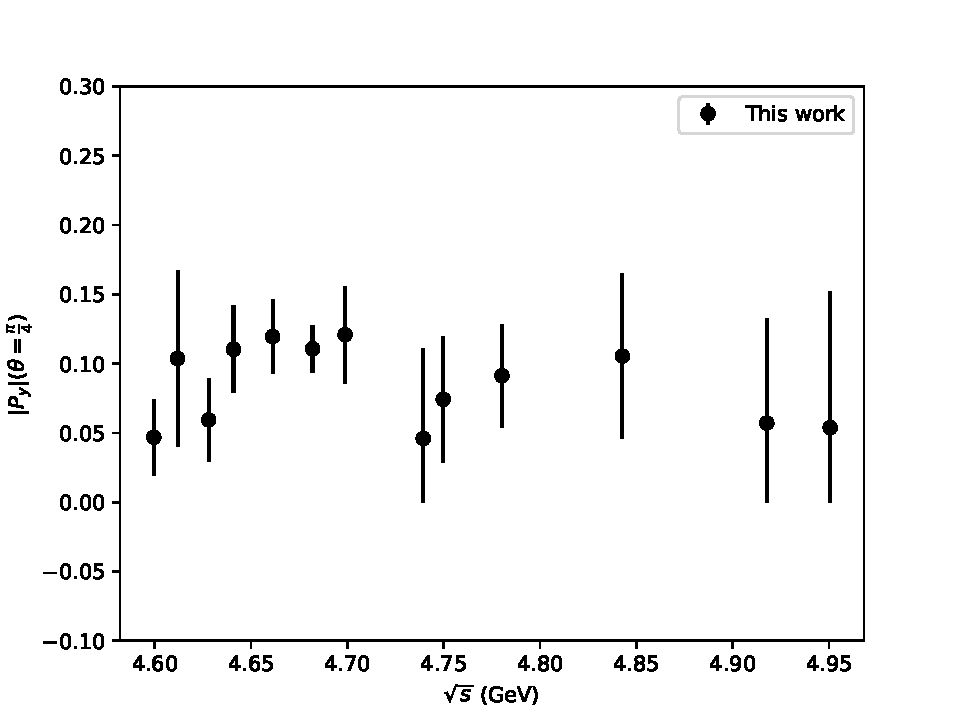
\includegraphics[width=0.80\textwidth]{figure/summary/max_Py.pdf}
    \caption{$| \frac{3}{2(3+\alpha_0)}\sqrt{1-\alpha_0^2}\sin\Delta_0\cos\theta_{\lcp}\sin\theta_{\lcp}|$ at all energy points. This value represents the maximal value of transverse polarization of $\lcp$.}
\label{fig:max_py}
\end{figure}

\begin{table}[H]
    \centering
    \caption{Results of FFs for each resonance in $\lcp \to p K^-\pi+$.}
    \label{tab:final-ff}
    \begin{tabular}{cccc}
    \hline\hline
    Resonance & FF (\%) \\\hline
    $ \Delta(1232)^{++} $ & 27.3 $\pm$ 1.0 $\pm$ 2.8 \\
    $ \Delta(1600)^{++} $ & 7.4 $\pm$ 1.7 $\pm$ 4.4 \\
    $ \Delta(1600)^{++} $ & 4.8 $\pm$ 1.7 $\pm$ 5.0 \\
    $ \Delta(1700)^{++} $ & 12.0 $\pm$ 1.4 $\pm$ 2.7 \\
    $ \bar{K}_{0}^{*}(1430) $ & 14.6 $\pm$ 2.8 $\pm$ 5.3 \\
    $ \bar{K}_{0}^{*}(700) $ & 2.6 $\pm$ 0.6 $\pm$ 3.6 \\
    $ \bar{K}^{*}(892) $ & 23.7 $\pm$ 1.3 $\pm$ 5.1 \\
    $ \Lambda(1405) $ & 4.4 $\pm$ 1.2 $\pm$ 2.5 \\
    $ \Lambda(1520) $ & 1.3 $\pm$ 0.2 $\pm$ 0.2 \\
    $ \Lambda(1600) $ & 4.8 $\pm$ 1.1 $\pm$ 1.7 \\
    $ \Lambda(1670) $ & 1.7 $\pm$ 0.3 $\pm$ 0.7 \\
    $ \Lambda(1690) $ & 0.9 $\pm$ 0.2 $\pm$ 0.5 \\
    $ \Lambda(2000) $ & 6.2 $\pm$ 0.5 $\pm$ 1.6 \\
\hline\hline
    \end{tabular}
\end{table}

\begin{table}[H]
    \centering
    \caption{Results of branching fractions of $\lcp \to \Delta(1232)^{++}K^-,\bar{K}^{*}(892)p, \Lambda(1520)\pi^+$. In this work, the first uncertainty is statistical one, the second one is systematical and the last one is from $\BR(\lcp \to pK^-\pi^+)$ in PDG~\cite{Workman:2022ynf}.}
    \label{tab:final-bf}
    \begin{tabular}{ccc}
    \hline\hline
    Decay& This work & PDG~\cite{Workman:2022ynf} \\\hline 
    $\BR(\lcp \to \Delta(1232)^{++}K^-)$ (\%) &  1.71$\pm$0.06$\pm$0.18$\pm$0.08 & 1.08$\pm$0.25 \\%27.34$\pm$1.03$\pm$2.00\\
    $\BR(\lcp \to \bar{K}^{*}(892)p)$ (\%)   &  2.23$\pm$0.12$\pm$0.48$\pm$0.10 & 1.95$\pm$0.27 \\%24.98$\pm$0.99$\pm$3.88\\
    $\BR(\lcp \to \Lambda(1520)\pi^+)$ (\%)  &  0.36$\pm$0.06$\pm$0.06$\pm$0.02 & 2.2 $\pm$ 0.5 \\%1.10$\pm$0.17$\pm$0.17\\
\hline\hline
    \end{tabular}
\end{table}


\begin{table}[H]
    \centering
    \caption{Comparison of $\alpha_0$ for this work, BAM-718 and previous measurement~\cite{BESIII:2017kqg,BESIII:2023rwv} in BESIII.}
    \label{tab:alpha0-comparison}
    \begin{tabular}{cccc}
    \hline\hline
dataset & This work &  BAM-718~\cite{ESIIImemo:LcDecayAsy} & Previous results~\cite{BESIII:2017kqg,BESIII:2023rwv} \\\hline
4600 & -0.23 $\pm$ 0.04 $\pm$ 0.00 & -0.22 $\pm$ 0.03 $\pm$ 0.00 & -0.20 $\pm$ 0.04 $\pm$ 0.02 \\
4612 & -0.23 $\pm$ 0.09 $\pm$ 0.02 & -0.17 $\pm$ 0.08 $\pm$ 0.00 & -0.26 $\pm$ 0.09 $\pm$ 0.01 \\
4626 & -0.15 $\pm$ 0.04 $\pm$ 0.00 & -0.22 $\pm$ 0.07 $\pm$ 0.00 & -0.21 $\pm$ 0.04 $\pm$ 0.01 \\
4640 & -0.06 $\pm$ 0.05 $\pm$ 0.00 & -0.06 $\pm$ 0.04 $\pm$ 0.00 & -0.09 $\pm$ 0.05 $\pm$ 0.01 \\
4660 & 0.03 $\pm$ 0.05 $\pm$ 0.01 & 0.01 $\pm$ 0.04 $\pm$ 0.00 & -0.02 $\pm$ 0.05 $\pm$ 0.01 \\
4680 & 0.15 $\pm$ 0.03 $\pm$ 0.00 & 0.10 $\pm$ 0.03 $\pm$ 0.00 & 0.15 $\pm$ 0.03 $\pm$ 0.01 \\
4700 & 0.33 $\pm$ 0.07 $\pm$ 0.00 & 0.31 $\pm$ 0.06 $\pm$ 0.01 & 0.34 $\pm$ 0.07 $\pm$ 0.01 \\
4740 & 0.42 $\pm$ 0.16 $\pm$ 0.03 & 0.36 $\pm$ 0.12 $\pm$ 0.01 & 0.49 $\pm$ 0.16 $\pm$ 0.03 \\
4750 & 0.41 $\pm$ 0.10 $\pm$ 0.00 & 0.35 $\pm$ 0.08 $\pm$ 0.00 & 0.42 $\pm$ 0.10 $\pm$ 0.01 \\
4780 & 0.19 $\pm$ 0.08 $\pm$ 0.01 & 0.17 $\pm$ 0.06 $\pm$ 0.01 & 0.17 $\pm$ 0.07 $\pm$ 0.01 \\
4840 & 0.35 $\pm$ 0.11 $\pm$ 0.01 & 0.28 $\pm$ 0.09 $\pm$ 0.02 & 0.38 $\pm$ 0.10 $\pm$ 0.01 \\
4914 & 0.69 $\pm$ 0.20 $\pm$ 0.01 & 0.62 $\pm$ 0.15 $\pm$ 0.02 & 0.62 $\pm$ 0.17 $\pm$ 0.01 \\
4946 & 0.52 $\pm$ 0.22 $\pm$ 0.04 & 0.74 $\pm$ 0.20 $\pm$ 0.04 & 0.63 $\pm$ 0.21 $\pm$ 0.01 \\
\hline\hline
    \end{tabular}
\end{table}

\begin{table}[H]
    \centering
    \caption{Comparison of $\Delta_0$ between this work and BAM-724~\cite{ESIIImemo:LcDecayAsy}. }
    \label{tab:delta0-compare}
    \begin{tabular}{cccc}
    \hline\hline
dataset & $\Delta_0$ in this work & $\Delta_0$ in BAM-718~\cite{ESIIImemo:LcDecayAsy} & Deviation ($\sigma$)\\\hline
4600 & -0.18 $\pm$ 0.08 $\pm$ 0.06 & -0.11 $\pm$ 0.07 $\pm$ 0.01 & 0.6 \\
4612 & -0.40 $\pm$ 0.21 $\pm$ 0.13 & -0.16 $\pm$ 0.15 $\pm$ 0.03 & 0.8 \\
4626 & -0.23 $\pm$ 0.10 $\pm$ 0.06 & -0.47 $\pm$ 0.13 $\pm$ 0.01 & 1.4 \\
4640 & -0.45 $\pm$ 0.09 $\pm$ 0.08 & -0.40 $\pm$ 0.08 $\pm$ 0.02 & 0.3 \\
4660 & -0.50 $\pm$ 0.10 $\pm$ 0.04 & -0.50 $\pm$ 0.09 $\pm$ 0.02 & 0.0 \\
4680 & -0.49 $\pm$ 0.06 $\pm$ 0.03 & -0.51 $\pm$ 0.06 $\pm$ 0.02 & 0.2 \\
4700 & -0.60 $\pm$ 0.13 $\pm$ 0.09 & -0.55 $\pm$ 0.12 $\pm$ 0.03 & 0.3 \\
4740 & 0.23 $\pm$ 0.29 $\pm$ 0.15 & -0.07 $\pm$ 0.19 $\pm$ 0.02 & 0.8 \\
4750 & -0.38 $\pm$ 0.20 $\pm$ 0.10 & -0.31 $\pm$ 0.14 $\pm$ 0.02 & 0.2 \\
4780 & -0.41 $\pm$ 0.15 $\pm$ 0.07 & -0.41 $\pm$ 0.13 $\pm$ 0.03 & 0.0 \\
4840 & -0.53 $\pm$ 0.22 $\pm$ 0.18 & -0.38 $\pm$ 0.16 $\pm$ 0.03 & 0.4 \\
4914 & 0.40 $\pm$ 0.44 $\pm$ 0.25 & -0.42 $\pm$ 0.26 $\pm$ 0.02 & 1.4 \\
4946 & -0.30 $\pm$ 0.43 $\pm$ 0.33 & -0.67 $\pm$ 0.39 $\pm$ 0.07 & 0.6 \\
\hline\hline
    \end{tabular}
\end{table}

\begin{figure}\centering
    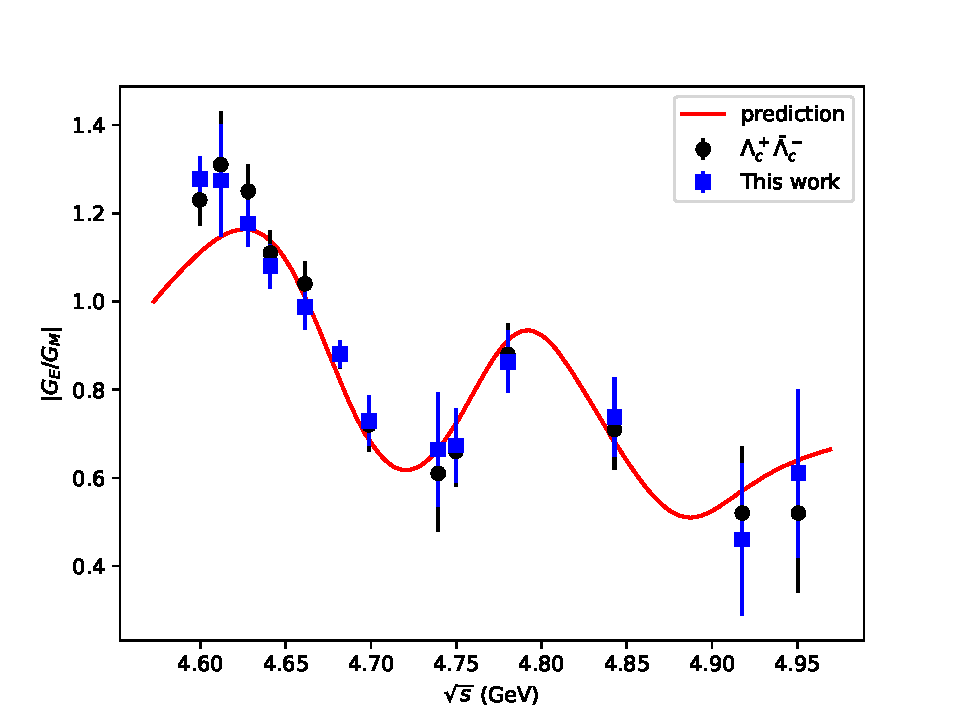
\includegraphics[width=0.45\textwidth]{figure/summary/comp_GE_GM_ratio.pdf}
    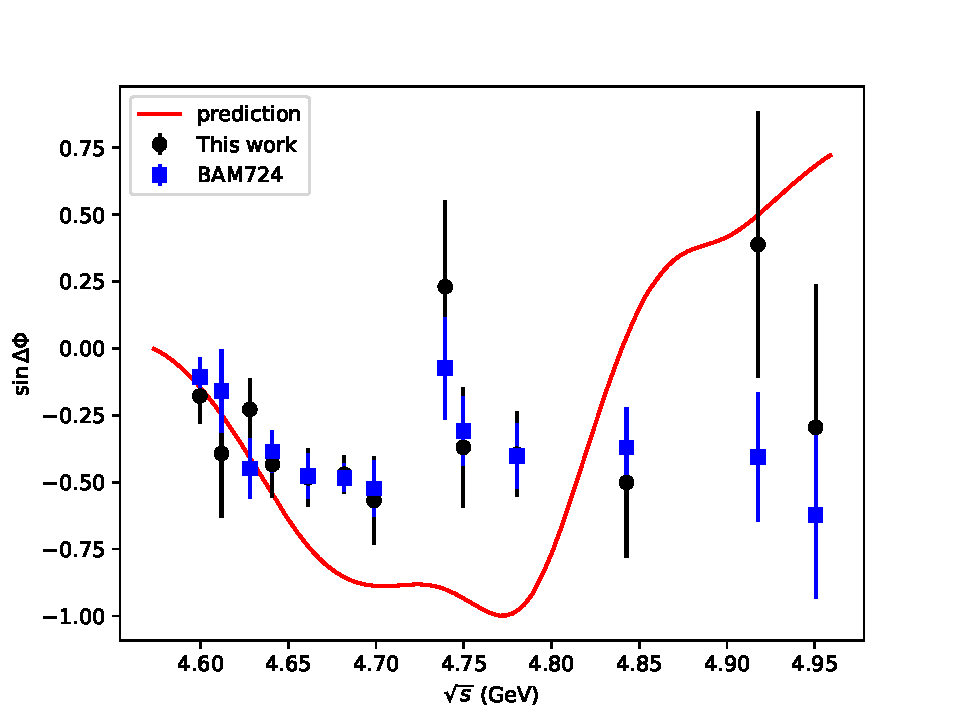
\includegraphics[width=0.45\textwidth]{figure/summary/comp_sinDeltaPhi.pdf}
    \caption{Comparison of $|G_E/G_M|$ (left) and $\sin\Delta_0$ (right) among this work, the previous measurement and theoretical predictions.}
\label{fig:comp_theory}
\end{figure}

All of these measurements will contribute to future investigations into the decay properties of charmed baryons, further enriching our comprehension of their underlying dynamics.


